\documentclass{beamer}
\usepackage{filecontents}

\begin{filecontents}{\jobname.bib}
	@article{derras2012adapting,
		title={Adapting the neural network approach to PGA prediction: An example based on the KiK-net data},
		author={Derras, Boum{\'e}di{\`e}ne and Bard, Pierre-Yves and Cotton, Fabrice and Bekkouche, Abdelmalek},
		journal={Bulletin of the Seismological Society of America},
		volume={102},
		number={4},
		pages={1446--1461},
		year={2012},
		publisher={Seismological Society of America}
	}

	
\end{filecontents}

\usepackage[backend=bibtex,style=numeric]{biblatex}
\addbibresource{\jobname.bib}

%construct dynamic page
\setbeamercovered{highly dynamic}
\newcounter{saveenumi}
\newcommand{\seti}{\setcounter{saveenumi}{\value{enumi}}}
\newcommand{\conti}{\setcounter{enumi}{\value{saveenumi}}}
\resetcounteronoverlays{saveenumi}

%set color and initial
\usetheme[progressbar=frametitle]{metropolis}
\definecolor{mygreen}{rgb}{.125,.5,.25}
\usecolortheme[named=mygreen]{structure}
\setbeamertemplate{frame numbering}[fraction]
\useoutertheme{metropolis}
\useinnertheme{metropolis}
\usefonttheme{metropolis}
\usecolortheme{spruce}
\setbeamercolor{background canvas}{bg=gray}

\title{Ground Shaking}
\subtitle{with Graph Nueral Network}
\author{Phiphat Chomchit}
\institute{Chiang Mai University}

\begin{document}
% Fill color in block
\metroset{block=fill}

	\begin{frame}
		\titlepage
	\end{frame}

	\begin{frame}[t]{Basic Seismic Knowlendge}

		\begin{enumerate}
			\item \textbf{Earthquake} is the sudden fracture and movement of rocks inside the Earth. 
			Part of the energy released produces seismic waves, like P, S, and surface waves that 
			travel outward in all directions from the point of initial rupture.
			\item \textbf{Hypocenter} or Focus the point below the epicenter at which an earthquake
			begins.
			\item \textbf{Epicenter} the point (map location) on the Earth’s surface directly above 
			the hypocenter or focus of an earthquake.
			\seti
		\end{enumerate}
		
	\end{frame}

	\begin{frame}[t]{stick-slip model}
		\begin{figure}
			\centering
			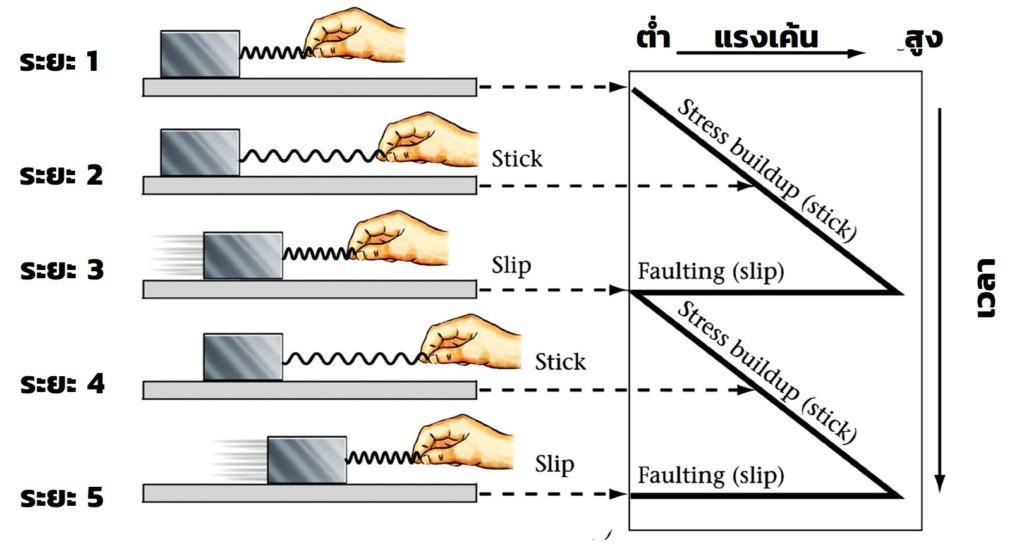
\includegraphics[scale=0.5]{stick.jpg}
			\caption{sick-slip model}
		\end{figure}
	\end{frame}

	\begin{frame}[t]{Basic Seismic Knowlendge}
		\begin{enumerate}
			\conti
			\item \textbf{P Wave} is the primary body wave; the first seismic wave detected by 
			seismographs; able to move through both liquid and solid rock. Also called compressional or 
			longitudinal waves, they compress and expand (oscillate) the ground back and forth in the 
			direction of travel, like sound waves that move back and forth as the waves travel from source 
			to receiver. P wave is the fastest wave.
			
			\item \textbf{S Waves} is shear waves that are secondary body waves that oscillate the ground 
			perpendicular to the direction of wave travel. They travel about 1.7 times slower than P waves. 
			Because liquids will not sustain shear stresses, S waves will not travel through liquids like water, 
			molten rock, or the Earth’s outer core. S waves produce vertical and horizontal motion in the 
			ground surface. 
			\seti
		\end{enumerate}
	\end{frame}

	\begin{frame}[t]{Body wave and surface wave}
		\begin{figure}
			\centering
			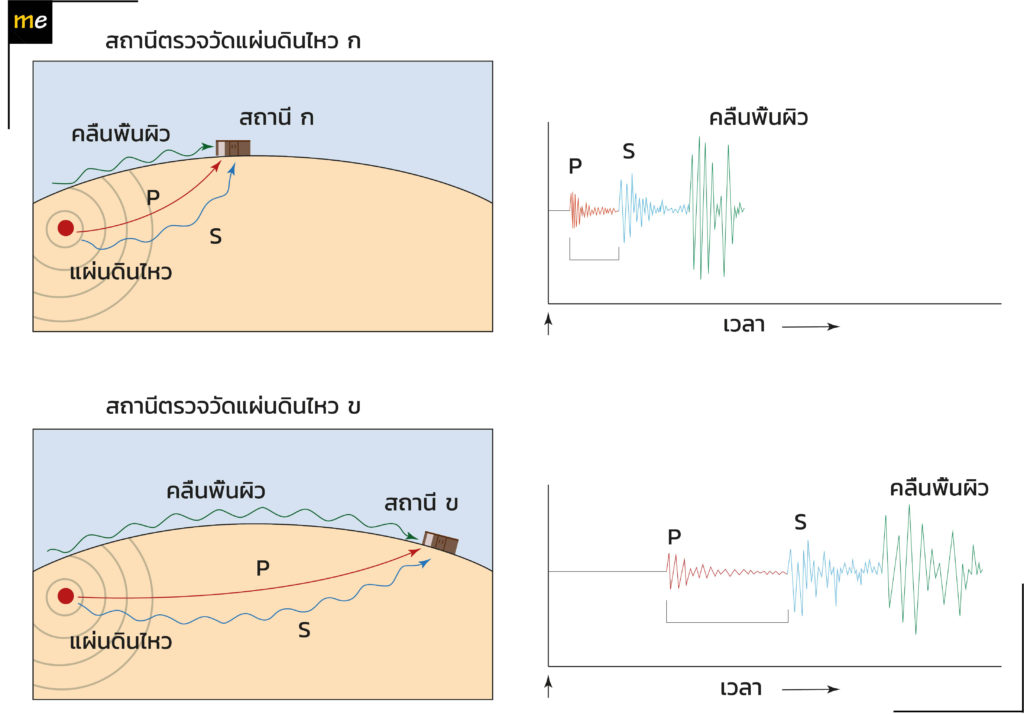
\includegraphics[scale=0.8]{station.jpg}
			\caption{P-wave, S-wave and surface wave}
		\end{figure}
	\end{frame}

	\begin{frame}[t]{Epicenter and Hypocenter}
		\begin{figure}
			\centering
			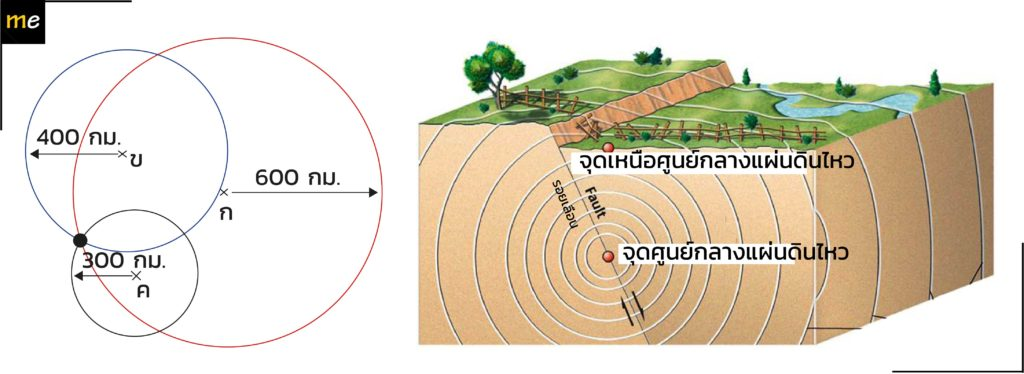
\includegraphics[scale=0.8]{velocity.jpg}
			\caption{Epicenter and Hypocenter}
		\end{figure}
	$V = \frac{S}{T}$
	
	$$T_p - T_s = \frac{S}{V_p} - \frac{S}{V_s}$$
	\end{frame}
	
	
	\begin{frame}[t]{Basic Seismic Knowlendge}
		\begin{enumerate}
			\conti
			\item \textbf{Peak Ground Acceleration} is a largest increase in velocity recorded by a particular station during 
			an earthquake. (Commonly called PGA) 
			\seti
		\end{enumerate}
	
		\begin{figure}
			\centering
			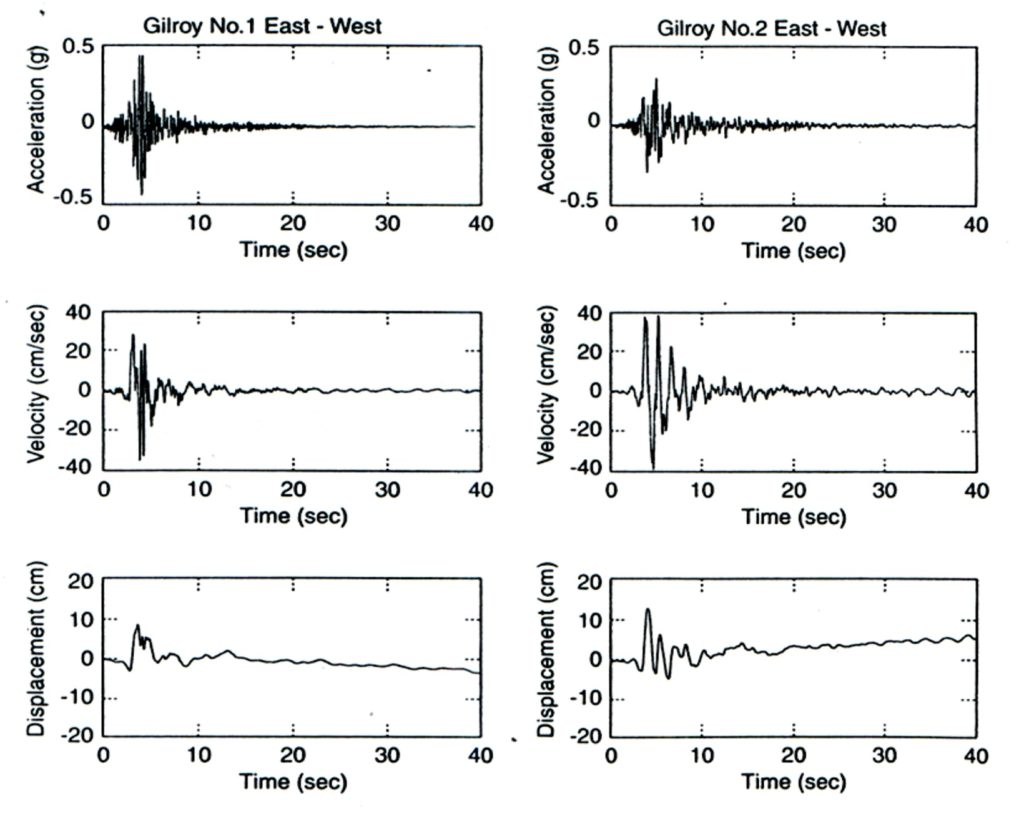
\includegraphics[scale=0.35]{pga.jpg}
			\caption{PGA, PGV, PGD}
		\end{figure}
	\end{frame}
	
	\begin{frame}[t]{Basic Seismic Knowlendge}
		\begin{enumerate}
			\conti
			\item \textbf{Attenuation} is decrease in wave size, or amplitude, away from source. When you 
			throw a pebble in a pond, it makes waves on the surface that move out from the place where 
			the pebble entered the water. The waves are largest where they are formed and get smaller as 
			they move away.
			\seti
		\end{enumerate}
	
		\begin{figure}
			\centering
			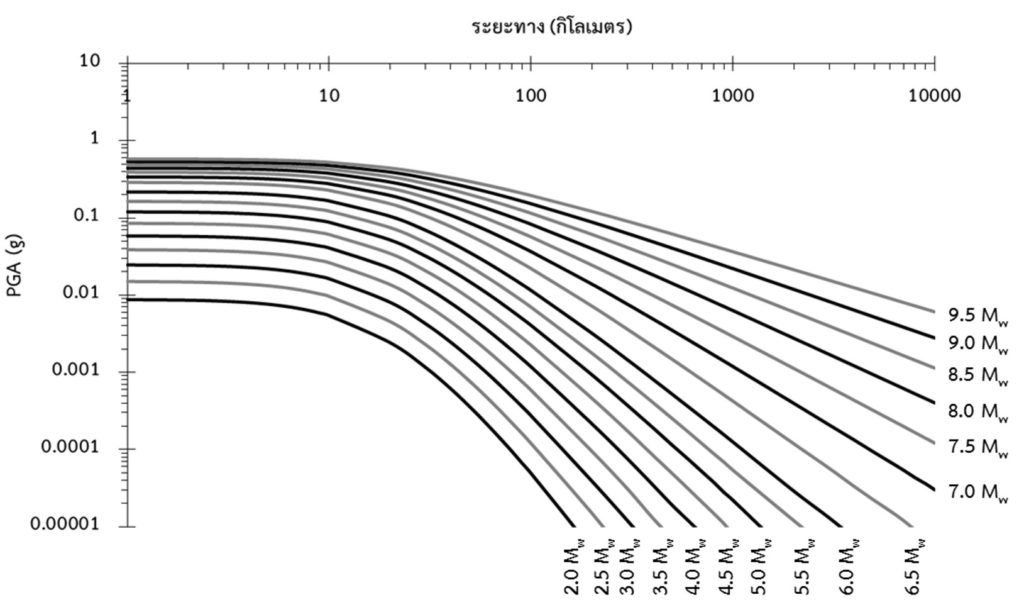
\includegraphics[scale=0.35]{anu.jpg}
			\caption{Attenuation}
		\end{figure}
	
	\end{frame}
	\begin{frame}[t]{Basic Seismic Knowlendge}
		\begin{enumerate}
			\conti
			\item \textbf{Ground motion prediction model (GMPEs)}, also called ground-motion models 
			(GMMs) and attenuation relations, estimate the shaking (strong ground motion) that may occur 
			at a site if an earthquake of a certain magnitude occurs at a nearby location.
		\end{enumerate}
	
		\begin{figure}
			\centering
			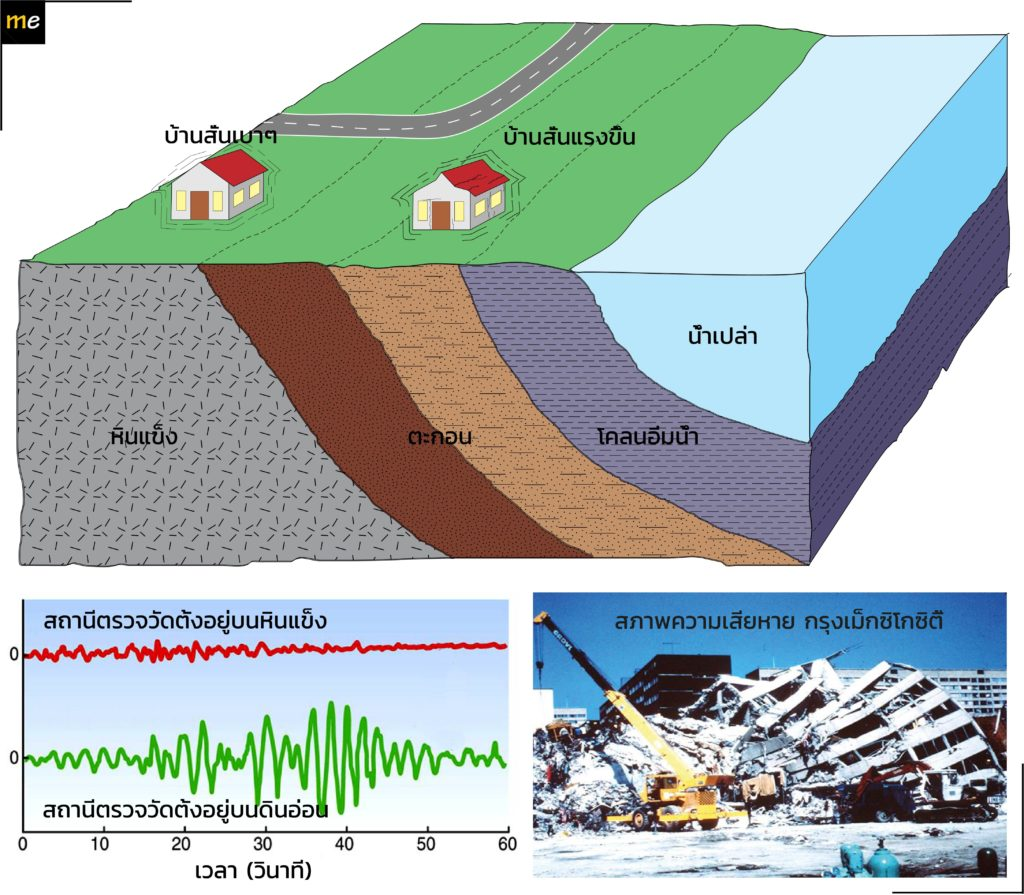
\includegraphics[scale=0.5]{shak.jpg}
			\caption{Ground Shaking}
		\end{figure}
	\end{frame}

	\begin{frame}[t]{Basic Seismic Knowlendge}
		\begin{enumerate}
			\conti
			\item \textbf{ShakeMap} The system is designed to combine instrumental measurements with information about local seismic site conditions and the earthquake source to estimate continuous shaking variations throughout a 
			spatial area. ShakeMap was implemented in other high-to-moderate-risk areas where rapid assessment of earthquakes is critical.
		\end{enumerate}
		\begin{figure}
			\centering
			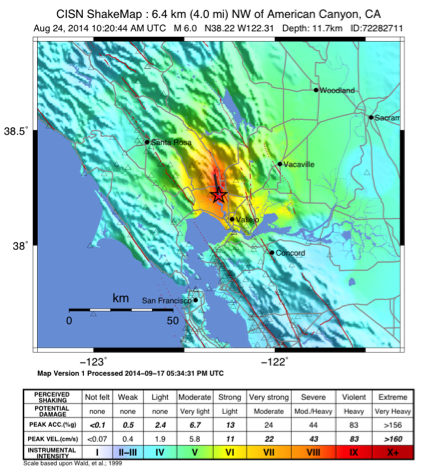
\includegraphics[scale=0.4]{example.png}
			\caption{Ground Shaking}
		\end{figure}
		
	\end{frame}
	\begin{frame}[t]{Review Papers}
		Why do we need machine learning?\\

		\vspace{10pt}
		\begin{enumerate}
			\item Parameters
			\begin{enumerate}
				\item Multilayer Perceptron
				\item Hybrid
				\item Genertic Programing
			\end{enumerate}
		\vspace{10pt}
			\item Waveform
			\begin{enumerate}
				\item Multilayer Perceptron
				\item Convolutional Neural Network
				\item Graph Neural Network
				\item Self Supervised Learning
			\end{enumerate}
		\end{enumerate}
	\end{frame}
	
	\begin{frame}[t]{Why do we need machine learning?}
		
	\end{frame}
	\begin{frame}[t]{Multilayer Perceptron}
	\end{frame}

	\begin{frame}[t]{Hybrid}
	\end{frame}

	\begin{frame}[t]{Genetic Programing}
	\end{frame}

	\begin{frame}[t]{Convolutional Neural Network}
	\end{frame}

	\begin{frame}[t]{Convolutional Neural Network}
	\end{frame}

	\begin{frame}[t]{Self Supervised Learning}
	\end{frame}

	\begin{frame}[t]{Focus on my work}
		Graph Neural Network
		
	\end{frame}

	\begin{frame}[t]{Focus on my work}
		Semi-Supervised Learning and Self-Supervised Learning.
	\end{frame}	

\end{document}